% !TEX root = ../main.tex
%
\chapter{Vorgeschlagenes Wissensgraph\-konstruktions\-verfahren}%
\label{sec:text2kg}

Auf Basis der vorgestellten Konzeptgraphen, CoreNLP und PSL wird im folgenden Kapitel ein Verfahren für die online Konstruktion eines Wissensgraphen aus natürlichsprachlichen Textnachrichten aufgebaut.
Der Fokus liegt dabei primär auf der generellen Architektur des Verfahrens.
Das Resultat ist also als Proof-of-Concept zu verstehen, auf dessen Basis praxistaugliche Systeme konzipiert werden können.

\begin{figure}[h]
	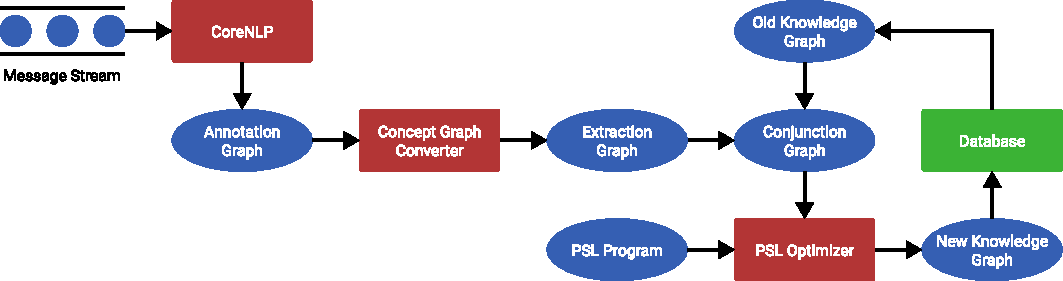
\includegraphics[width=\textwidth]{gfx/text2kg/architecture.pdf}
	\caption{Grobes Architekturdiagramm der Konstruktionspipeline}\label{fig:text2kg:architecture}
\end{figure}
Das im Folgenden vorgestellte Verfahren folgt einem dreistufigen Pipeline-Modell:
\begin{enumerate}
	\item Mittels CoreNLP wird eine eintreffende Textnachricht in einen Abhängigkeitsgraphen transformiert.
	\item Der resultierende Abhängigkeitsgraph wird in einen sog.\ Extraktionsgraphen umgewandelt.
		Hierbei handelt es sich um einen Konzeptgraphen, der den Inhalt der Nachricht formal repräsentiert.
	\item Der Extraktionsgraph wird mit dem bestehenden Wissensgraphen verschmolzen.
		Dies entspricht der Konjuktion der durch die beiden Graphen repräsentierten logischen Ausdrücke.
		Der resultierende Konjunktionsgraph wird als Eingabe für ein PSL-Programm verwendet, welches auf Basis des hinzugekommenen Wissens neue Beziehungen im Wissensgraphen inferiert.
\end{enumerate}
Die Beschreibung dieser Pipeline erfolgt in vier Abschnitten.
In \treft{sec:text2kg:implementation} wird kurz die technische Umsetzung erläutert.
\treft{sec:text2kg:ontology} beschreibt anschließend die Ontologie der konstruierten Wissensgraphen.
Nach diesen strukturellen Betrachtungen wird schließlich in \treft{sec:text2kg:nlp} und \treft{sec:text2kg:psl} die Transformation von Text zu Extraktionsgraph, bzw.\ von Extraktionsgraph zu Wissensgraph beschrieben.

\section{Implementation}%
\label{sec:text2kg:implementation}

Das in den folgenden Abschnitten beschriebene Verfahren wurde im Rahmen dieser Arbeit prototypisch implementiert.
Bei der Wahl der hierfür verwandten Technologien wurde darauf Wert gelegt, dass eine möglichst nahtlose Integration der Komponenten möglich ist.
Sowohl CoreNLP~\cite{CoreNLP} als auch die PSL-Referenzimplementation~\cite{PSL} sind JVM-Bibliotheken.
Diese Arbeit wurde daher ebenfalls in einer JVM-Sprache implementiert.

Hierfür wurde Clojure gewählt, ein moderner Lisp-1-Dialekt, mit einem Fokus auf funktionale Programmierung, unveränderliche Datenstrukturen und gleichzeitiger Interoperabilität mit objektorientierten Bibliotheken.
Andere JVM-Sprachen, wie z.~B. Java, Scala oder Groovy, wurden ausgeschlossen, da sie sich während des Entwicklungsprozesses als hinderlich erwiesen haben.
Der Hauptgrund hierfür ist, dass CoreNLP bei der Initialisierung diverse Modelle laden muss.
Bei Verwendung eines modernen Desktop-Rechners benötigt dies ca.~20 Sekunden, auf langsamerer Hardware teils mehrere Minuten;
diese Wartezeiten waren ein stark verlangsamender Faktor beim entwickeln.
Da Clojure ein Lisp ist, unterstützt es traditionsgemäß \textit{REPL Driven Development}.
Statt nach jeder Änderung die Anwendung neu zu starten und die Modelle erneut zu laden, kann so lediglich der geänderte Bytecode in den laufenden Prozess injiziert werden;
die geladenen Modelle bleiben dabei im Speicher und die Änderung kann ohne weitere Wartezeit getestet werden.
Durch die Wahl von Clojure konnte die Entwicklung deutlich beschleunigt werden.

\section{Wissensgraphontologie}%
\label{sec:text2kg:ontology}

Bevor Wissensgraphen konstruiert werden können, muss spezifiziert sein, wie genau diese aussehen sollen.
Um komplexe logische Beziehungen ausdrücken zu können, wird die bereits vorgestellte Konzeptgraph-Struktur verwendet.
Dabei bleibt allerdings offen, welche Prädikate vorkommen können und welche Bedeutung sie haben.
Außerdem ist unklar, wie mit Konzeptgraphen modale Aussagen ausgedrückt werden.
Damit aus einem Konzeptgraphen ein Wissensgraph wird, muss eine Ontologie gegeben sein, welche diese offenen Punkte schließt.
Im Folgenden wird beschrieben, wie genau die in dieser Arbeit verwendete Ontologie aufgebaut ist.

\subsection{Verwendete Prädikate}%
\label{sec:text2kg:ontology:pred}

\subsection{Modale Kontexte}%
\label{sec:text2kg:ontology:modal}

Im zweiten Schritt wird nun geklärt, wie Modalität repräsentiert wird.
Beispiele für modale Aussagen sind:
\begin{center}
	\textit{``I {\color{blau}think} that {\color{rot}the book is good}.''}\\
	\textit{``{\color{rot}I} {\color{blau}don't want} to {\color{rot}go to the beach}.''}
\end{center}
Die beiden Teilaussagen \textit{\color{rot}``the book is good''} und \textit{\color{rot}``I go to the beach''} sind offensichtlich nicht unbedingt wahr, sondern beschreiben Möglichkeiten, die in Abhängigkeit von \textit{\color{blau}think} bzw.\ \textit{\color{blau}don't want} wahr oder falsch werden könnten.
Ob die Aussagen wahr werden, hängt davon ab, inwiefern das Denken oder Wollen einer Person mit der Realität übereinstimmt.
Dies ist je nach Person stark verschieden; manche tendieren dazu die allgemein als wahr akzeptierten Aussagen zu denken bzw.\ entsprechend ihrer Wünsche zu handeln, andere nicht.

Um derartige Möglichkeiten und Notwendigkeiten direkt zu repräsentieren, reichen die vorgestellten Konzeptgraphen mit Negationskontexten nicht aus.
Sowa hat dieses Problem ebenfalls erkannt und daher weitere Kontexttypen eingeführt.
Die Beschreibung dieser zusätzlichen Kontexttypen ist allerdings oftmals zu unpräzise für eine eindeutige Übersetzung in die Prädikatenlogik.
Aufbauend auf Sowas Ideen wird in dieser Arbeit daher eine abgeschwächte Variante modaler Kontexte eingeführt, die die Übersetzbarkeit in die Prädikatenlogik erster Ordnung bewahrt.
Da die zuvor vorgestellten Konzeptgraphen bereits vollständig und korrekt sind, handelt es sich bei diesen modalen Kontexten also lediglich um eine Kurzschreibweise.

Insgesamt gibt es durch die Erweiterung um modale Kontexe nun folgende vier Kontexttypen:
\begin{multicols}{2}
	\flushleft\begin{enumerate}
		\item Positiver Aktualkontext
		\item Negativer Aktualkontext
		\item Positiver Möglichkeitskontext
		\item Negativer Möglichkeitskontext
	\end{enumerate}
\end{multicols}
Die modale Notwendigkeit hat keine eigenen Kontexttypen erhalten, um konsistent zur Quantisierung in Konzeptgraphen zu bleiben.
So, wie der Allquantor in Konzeptgraphen durch Negation der negierten existenzquantisierten Aussage ausgedrückt wird, wird die Notwendigkeit durch Negation der negativen Möglichkeit ausgedrückt.

Da es nun vier Kontexttypen gibt, muss die Konzeptgraphsyntax leicht angepasst werden, um zwischen den verschiedenen Typen differenzieren zu können:
\begin{figure}[h]
	\centering
	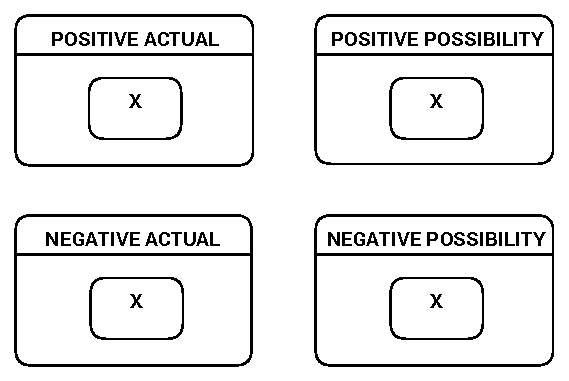
\includegraphics[scale=0.6]{gfx/text2kg/contextTypes.pdf}
	\caption{Konzeptgraphsyntax für modale Kontexte}\label{fig:text2kg:contextTypes}
\end{figure}

\paragraph{Positiver Aktualkontext}
Dieser Kontexttyp hat keinen Einfluss auf die Bedeutung der enthaltenen Knoten.
Er entspricht in etwa der Klammerung in der Prädikatenlogik.
Das \textit{Sheet of Assertion}~$\top$ ist ein solcher Kontext, abgesehen davon tauchen positive Aktualkontexte allerdings nicht auf;
sie werden hier lediglich der Vollständigkeit halber erwähnt.
\begin{align}
	\vcenter{\hbox{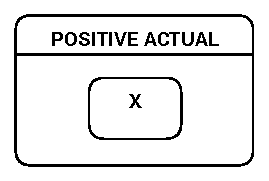
\includegraphics[scale=0.6]{gfx/text2kg/positiveActual.pdf}}}
	\Leftrightarrow
	\vcenter{\hbox{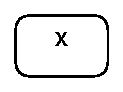
\includegraphics[scale=0.6]{gfx/text2kg/x.pdf}}}
	\Leftrightarrow
	\exists x: label(x, \text{``X''})
\end{align}

\paragraph{Negativer Aktualkontext}
Entspricht dem bisherigen Negationskontext.
\begin{align}
	\vcenter{\hbox{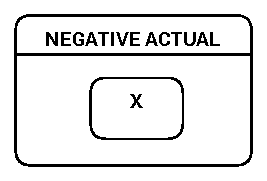
\includegraphics[scale=0.6]{gfx/text2kg/negativeActual.pdf}}}
	\Leftrightarrow
	\lnot \exists x: label(x, \text{``X''})
\end{align}

\paragraph{Positiver Möglichkeitskontext}
Dieser Kontexttyp bildet die modale Möglichkeit ab.
Um die Mächtigkeit der Prädikatenlogik beizubehalten, wird hierfür keine fundamental neue Struktur eingeführt.
Es wird stattdessen die Tatsache ausgenutzt, dass sich die modalen Operatoren gemäß der Mögliche-Welten-Interpretation analog zu den prädikatenlogischen Quantoren verhalten.
\begin{align*}
	{\color{rot}\square} P(x)\ &\Leftrightarrow \lnot {\color{blau}\lozenge} \lnot P(x) \\
	{\color{rot}\forall} w: world(w) \rightarrow P_w(x)\ &\Leftrightarrow \lnot {\color{blau}\exists} w: world(w) \land \lnot P_w(x) \numberthis
\end{align*}
Die Aussage \textit{``$P(x)$ gilt notwendigerweise''}, wird also als \textit{``Es gibt keine Welt $w$ in der $P_w(x)$ nicht gilt''} aufgefasst.
Statt von Welten, wird in modalen Konzeptgraphen allerdings von Kontexten gesprochen.

\paragraph{Negativer Möglichkeitskontext}
Lediglich eine Kurzschreibweise für einen positiven Möglichkeitskontext der einen negativen Aktualkontext umgibt.

\section{NLP-Phase}%
\label{sec:text2kg:nlp}

\section{Graphkonstruktionsphase}%
\label{sec:text2kg:psl}
